\chapter{Implementación y resultados}  \label{implementations_sec}

\section{Especificaciones}

El diseño fue implementado en una FPGA Xilinx Artix-35T (xc7a35ticsg324-1L)
utilizando las herramientas del software Xilinx Vivado Design Suite 2017.4. Se
trabajó con un clock de referencia de $100$ MHz, y el script para el
pre-procesamiento y el post-procesamiento fueron escritos en Python 2.7. 

Tanto los coeficientes del kernel como el correspondiente lote de imagen, se
cargan a la placa a través del puerto UART. Si bien esta vía es lenta con
respecto al tiempo de procesamiento, se optó por utilizarla debido a su
simplicidad y al bajo consumo de recursos comparado a otros medios de
transmisión.

En lo que refiere a representación de datos, como se explica en la
sección~\ref{fixedpoint}, se trabajó con aritmética en punto fijo, con una
resolución de $U(8,0)$ para la imagen de entrada y salida (imagen procesada), y
$S(8,7)$ para el kernel.

\section{Verificación}

Para verificar el comportamiento del sistema. se armaron diferentes kernels
en Python, y se aplicaron los mismos a una imagen de prueba. Luego, 
se filtró a la imagen con los mismos kernels  pero utilizando la FPGA
Los kernels que se utilizaron fueron: identidad $[0, 0, 0; 0, 1, 0; 0, 0,
0]$ sharpening $[0, -1, 0; -1, 5, -1; 0, -1, 0]$ y embossing $[-2, -1, 0; -1,
0, 1; 0, 1, 2]$. La figura~\ref{images_py_po} los resultados obtenidos.

\begin{figure}[!t]
\centering
\subfloat[][Identidad]{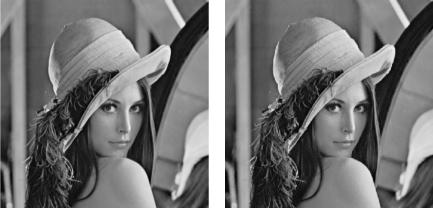
\includegraphics[scale=1.1]{identity_c}
  \label{fig:identity}}
\hfil
\subfloat[][Sharpening]{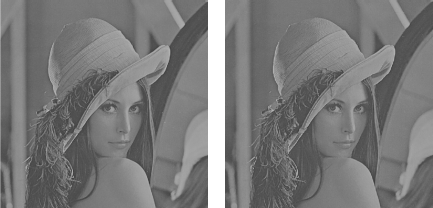
\includegraphics[scale=1.1]{shaped_c}
  \label{fig:share}}
\hfil
\subfloat[][Embossing]{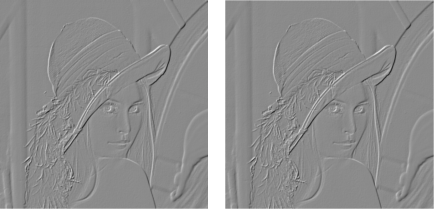
\includegraphics[scale=1.1]{emboss_c2}
\label{fig:embossing}}
\caption{Comparación de resultados: A la izquierda, la imagen procesada en una CPU usando python y, a la
  izquierda, la misma imagen procesada con el módulo en la FPGA.}
\label{images_py_po}
\end{figure}

\section{Utilización de recursos}

La arquitectura se sintetizó para diferentes grados de paralelismo. La tabla
Tabla~\ref{res_table} muestra la complejidad del módulo y el microprocesador en
la FPGA con y sin el uso de DSP respectivamente, medida por la utilización de
recursos. Se ve un incremento lineal acorde al grado de paralelismo en el
sistema. Debido a las limitaciones de la FPGA utilizada, se llegó a instanciar
$8$ $MAC$ $units$ para que operen en pparalelo con DSP, y $24$ sin el uso de DSP
pero con una utilización de $LUTs$ más intensiva.

\begin{table}
% increase table row spacing, adjust to taste
\renewcommand{\arraystretch}{1.3}
% if using array.sty, it might be a good idea to tweak the value of
% \extrarowheight as needed to properly center the text within the cells
\caption{Utilización de recursos con y sin DSP.}
\label{res_table}
\centering
% some packages, such as mdw tools, offer better commands for making tables
% than the plain latex2e tabular which is used here.
\begin{tabular}{|c|c|c|c|c|c|c|}
  \hline
  & \multicolumn{3}{c|}{\textbf{With DSP [N](\%)}} & \multicolumn{3}{c|}{\textbf{Without DSP [N](\%)}} \\ \hline
  \textbf{P}  & \textbf{DSP}            & \textbf{LUT}        & \textbf{BRAM}       & \textbf{DSP}         & \textbf{LUT}           & \textbf{BRAM}         \\ \hline
  2  & 20(22)         & 1845(9)    & 10(20)     & ---         & 3168(15)      & 10(20)         \\ \hline
  4  & 40(44)         & 2022(10)   & 11(22)     & ---         & 4627(22)      & 11(22)         \\ \hline
  6  & 60(67)         & 2175(10)   & 12(24)     & ---         & 6063(29)      & 12(24)         \\ \hline
  8  & 80(89)         & 2448(12)   & 13(26)     & ---         & 7756(37)      & 13(26)         \\ \hline
  10 & ---            & ---        & ---        & ---         & 9328(45)      & 14(28)         \\ \hline
  12 & ---            & ---        & ---        & ---         & 10917(52)     & 15(30)         \\ \hline
  24 & ---            & ---        & ---        & ---         & 20209(97)     & 21(42)         \\ \hline
\end{tabular}           
\end{table}

También se realizó una comparación, mostrada en la figura~\ref{bram_n}, entre la
utilización de BRAM estimada, y los resultados obtenidos de la síntesis. Se
efectuó una normalización con respecto al porcentaje de utilización de BRAM
dividiendo el máximo valor de porcentaje de utilización, y considerando que la
instancia del microblaze ya ocupa $18\%$ de los recursos BRAM.
Puede observarse que el comportamiento lineal anticipado por los
cálculos teóricos, es consistente con los resultados de la síntesis.

\begin{figure}
\centering
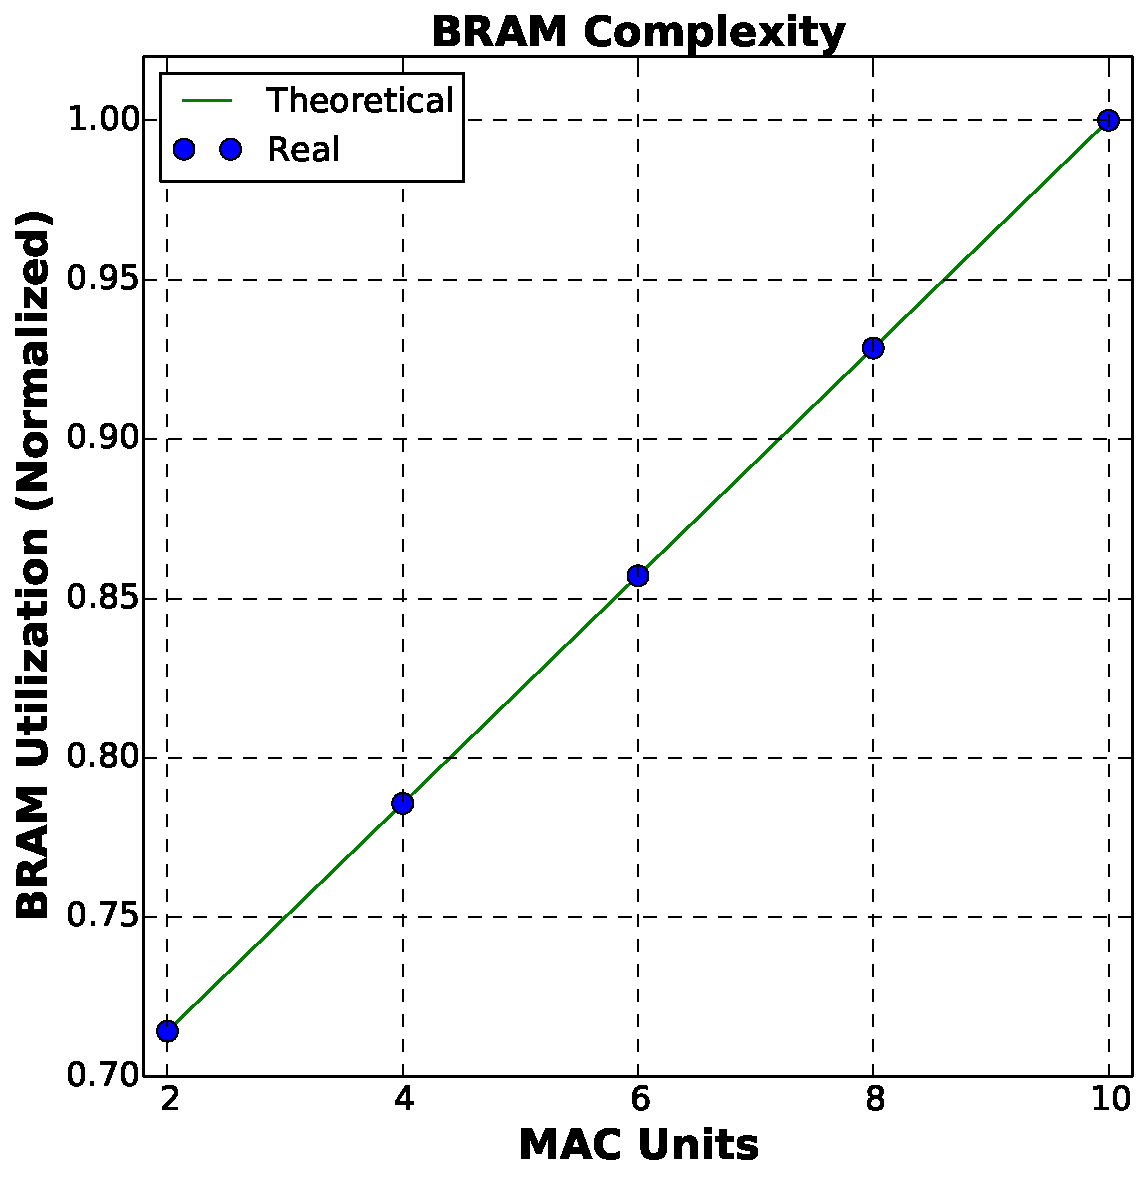
\includegraphics[scale=0.5]{BRAM_c2}
\caption{Curva normalizada para la utilización de los recursos de BRAM.}
\label{bram_n}
\end{figure}

\section{Throughput}

Considerando únicamente la operación de convolución, es decir, no teniendo en
cuenta el tiempo necesario para cargar la imagen en memoria, se obtiene un pixel
por ciclo de clock ($100$ Mhz) por cada $MAC$ $Unit$ instanciada. 

El throughput incrementa linealmente con el grado de paralelismo. La tabla
\ref{conv_tp} muestra el throughput obtenido para los diferentes grados de
paralelismo.

\begin{table}
% increase table row spacing, adjust to taste
\renewcommand{\arraystretch}{1.3}
% if using array.sty, it might be a good idea to tweak the value of
% \extrarowheight as needed to properly center the text within the cells
\caption{Throughput obtenido en lo que respecta a la convolución.}
\label{conv_tp}
\centering
% some packages, such as mdw tools, offer better commands for making tables
% than the plain latex2e tabular which is used here.
\begin{tabular}{|c|c|c|}
 \hline
  \textbf{Parallelism}  &    \textbf{Processing Speed [Mp/s]}  \\ \hline
          2             &                     200              \\ \hline
          4             &                     400              \\ \hline
          8             &                     800              \\ \hline
\end{tabular}           
\end{table}